\documentclass[a4paper,11pt]{article}
\usepackage[utf8]{inputenc}
\usepackage{amssymb}
\usepackage{amsmath} 
\usepackage{enumerate}
\usepackage{tikz}

% \DeclareMathOperator*{\argmax}{arg\!\max}
\DeclareMathOperator*{\argmin}{arg\!\min}
\DeclareMathOperator*{\var}{var}
\newcounter{exercise}
\setcounter{exercise}{0}
\newcounter{subexercise}
\newcommand*{\exercise}[1][]{
  \subsection*{Exercise
    \ifx/#1/\stepcounter{exercise}\arabic{exercise}
    \else#1\fi
  }
  \setcounter{subexercise}{0}
}
\newcommand*{\subexercise}[1][]{
  \par{
    \noindent\textbf{\ifx/#1/\protect\stepcounter{subexercise}\alph{subexercise}\else#1\fi.\quad}
  }
}
\title{Chapter 9}
\author{stevenjin8}
\date{\today}

\begin{document}
  \maketitle

  \section*{Comments}
  I found this chapter to be quite confusing, mostly due to the inconsistent notation. In section
  17.4.2, the author introduces $\psi_t(j) = p(\mathbf{x}_t|z_t=j)$. However, from section 17.4.2
  onwards, he uses $\phi$ instead of $\psi$. I also found it confusing that in section 17.5, the
  author switched $\boldsymbol{\Psi}$ for $\mathbf{A}$

  Another point of confusion was section 17.4.3.2. I spent a lot of time gazing at 17.62-17.63 and
  came to the conclusion that equation 17.63 is wrong (despite 17.66 being correct). I believe that
  the correct derivation should be
  \begin{align*}
    \xi_{t-1, t}(i, j) &\triangleq p(z_{t-1}=i, z_t=j| \mathbf{x}_{1:T}) \\
    &\propto p(\mathbf{x}_{t:T}, z_{t-1}=i, z_{t-1}=i | \mathbf{x}_{1:t-1}) \\
    &= p(\mathbf{x}_t, \mathbf{x}_{t+1:T}|z_{t-1}=i, z_t=j)
    p(z_{t-1}=i, z_t=j |\mathbf{x}_{1:t-1}) \\
    &= p(\mathbf{x}_t | z_{t}=j) p(\mathbf{x}_{t+1:T}|z_t=j) p(z_t=j|z_{t-1}=i)
    p(z_{t-1}=i|\mathbf{x}_{1:t-1}) \\
    &= \phi_{t}(j) \beta_t(j) \psi(i, j) \alpha_{t-1}(i).
  \end{align*}

  \setcounter{exercise}{2}
  \section*{Exercises}
  \exercise
  \subexercise \begin{center}
    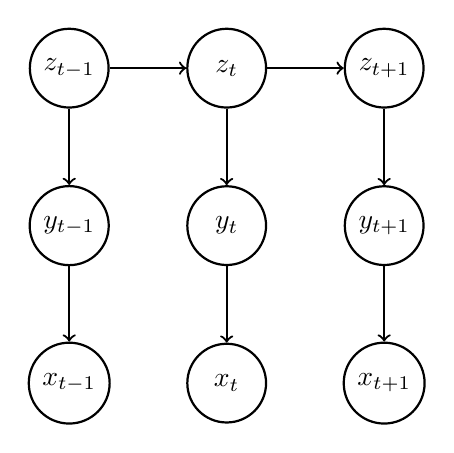
\begin{tikzpicture}[node distance={20mm}, thick, main/.style = {draw, circle, minimum size=10mm}]
      \node[main] (1) {$z_{t-1}$}; 
      \node[main] (2) [right of=1] {$z_t$};
      \node[main] (3) [right of=2] {$z_{t+1}$}; 
      \node[main] (4) [below of=1] {$y_{t-1}$}; 
      \node[main] (5) [below of=2] {$y_t$}; 
      \node[main] (6) [below of=3] {$y_{t+1}$}; 
      \node[main] (7) [below of=4] {$x_{t-1}$}; 
      \node[main] (8) [below of=5] {$x_t$}; 
      \node[main] (9) [below of=6] {$x_{t+1}$}; 

      \draw[->] (1) -- (2); 
      \draw[->] (2) -- (3); 
      \draw[->] (1) -- (4); 
      \draw[->] (2) -- (5); 
      \draw[->] (3) -- (6); 
      \draw[->] (4) -- (7); 
      \draw[->] (5) -- (8); 
      \draw[->] (6) -- (9); 
    \end{tikzpicture}
  \end{center}

  \subexercise
    \begin{align*}
      Q(\boldsymbol{\theta}, \boldsymbol{\theta}^{old}) &= \mathbb{E}\left[
        \log p(\mathcal{D}|\boldsymbol{\theta})
        | \mathcal{D}, \boldsymbol{\theta}^{old}\right
      ] \\
      &= \sum\limits_{i=1}^{N} \sum\limits_{t=1}^{N_i}
      \mathbb{E} [
        \log p(\mathbf{x}_{t,i} | y_i) + \log p(y_{t,i} | z_{t,i}) + \log p(z_{t,i} | z_{t,i-1})
      ] \\
      &= \sum\limits_{i=1}^{N} \sum\limits_{t=1}^{N_i}
      \mathbb{E} [
        \log \mathcal{N}(\mathbf{x}_{t,i} | \boldsymbol{\mu}_{y_i, z_i}, \boldsymbol{\Sigma}_{y_i, z_i})
        + \log w_{y_i, z_i}
        + \log \Phi_{z_{t,i-1}, z_{t, i}}
      ].
    \end{align*}
  \subexercise
    \begin{align*}
      \boldsymbol{\mu}_{j, k} &= \frac{
        \sum\limits_{i=1}^{N} \sum\limits_{t=1}^{N_i}
        \mathbf{x}_{t,i} p(y_{t,i}=j, z_{t,i}=j | \mathbf{x}_i)
      }{\sum\limits_{i=1}^{N} \sum\limits_{t=1}^{N_i} p(y_{t,i}=j, z_{t,i}=k | \mathbf{x}_i)} \\
      \boldsymbol{\Sigma}_{j,k} &= \frac{
        \sum\limits_{i=1}^{N} \sum\limits_{t=1}^{N_i}
        \mathbf{x}_{t,i} \mathbf{x}_{t,i}^T p(y_{t,i}=j, z_{t,i}=j | \mathbf{x}_i)
      }{\sum\limits_{i=1}^{N} \sum\limits_{t=1}^{N_i} p(y_{t,i}=j, z_{t,i}=k | \mathbf{x}_i)}
      - \boldsymbol{\mu}_{j,k} \boldsymbol{\mu}_{j,k}^T \\
      w_{jk} &= \frac{
        \sum\limits_{i=1}^{N} \sum\limits_{t=1}^{N_i} p(y_{t,i}=j, z_{t,i}=j | \mathbf{x}_i)
      }{
        \sum\limits_{i=1}^{N} \sum\limits_{t=1}^{N_i} p(z_{t,i}=k | \mathbf{x}_i)
      } \\
      \phi_{j,k} &= \frac{
        \sum\limits_{i=1}^{N} \sum\limits_{t=2}^{N_i} p(z_{t-1,i}=k, z_{t,i}=j| \mathbf{x}_i)
      }{
        \sum\limits_{i=1}^{N} \sum\limits_{t=1}^{N_i} p(z_{t-1,i}=j| \mathbf{x}_i)
      } \\
      \pi_{j} & \propto \sum\limits_{i=1}^{N} p(z_{1,i}=j | \mathbf{x}_i),
    \end{align*}
    where the probabilities are parameterized with $\boldsymbol{\theta}^{old}$. We can find
    $p(z_t| \mathbf{x})$ by using results from section 17.4 and equation 17.25. We can find
    $p(y_t|z_t, \mathbf{x})$ using Bayes' rule.

  \exercise
    The idea is the same as the previous exercise, except that
    \begin{align*}
      \boldsymbol{\mu}_m &= \frac{
        \sum\limits_i \sum\limits_t \sum\limits_k \mathbf{x}_{t,i} p(y_{t, i}=m, z_{t,i}=k | \mathbf{x}_i)
      }{
        \sum\limits_i \sum\limits_t \sum\limits_k p(y_{t, i}=m, z_{t,i}=k | \mathbf{x}_i)
      } \\
      \boldsymbol{\Sigma}_m = &= \frac{
        \sum\limits_{i=1}^{N} \sum\limits_{t=1}^{N_i}
        \mathbf{x}_{t,i} \mathbf{x}_{t,i}^T p(y_{t,i}=j, z_{t,i}=j | \mathbf{x}_i)
      }{
        \sum\limits_{i=1} \sum\limits_{t=1} \sum\limits_j p(y_{t,i}=j, z_{t,i}=k | \mathbf{x}_i)
      } - \boldsymbol{\mu}_m \boldsymbol{\mu}_m^T
    \end{align*}
\end{document}
